\cleardoublepage
\chapter{Video Compression Systems}\label{chap:av1}

%%%%%%%%%%%%%%%%%%%%%%%%%%%%%%%%%%%%%%%%%%%%%%%%%%%%%%%%%%%%%%%%%%%%%%%%%%%%%%
\section{Basic Principles}

\emph{Video Compression Systems} have been in development for approximately forty years, with the first video codec, \emph{H.120}, being released in 1984. It was composed of basic operations, which didn't correlate to good compression performances. This has lead to a quick downfall of its usage, being aggravated by the release of the \emph{H.261} standard by 1984.

However, the building blocks on which later standards were based are the same as in the first generations, i.e., the strategies implemented on newer standards exploit the same \emph{redundancies} as previous, less efficient, codecs.

By redundancies, it is meant disposable information to the playback of an image sequence. This concept is the key of video compression. Throughout the years, the enhancement of video codecs was based on the improving the algorithms which can reliably represent a video, while maintaining the least of the original information. In other words, the video sequence is analyzed for predictable/identifiable characteristics, e.g. the movement of a subject or the edge of an object, calculates strategies of predicting nearby pixel values through that information and disposes the unused information. This process is mentioned as \emph{redundancy removal}.

This way, to have a better understanding of the functioning behind video codecs, the mentioned redundancies, and respective origins, are presented. Most of such have origin on the way humans perceive vision, being this the first topic of this chapter.

%%%%%%%%%%%%%%%%%%%%%%%%%%%%%%%%%%%%%%%
\subsection{Human Visual System} \label{ssec:hvs}

%\todo[inline,color=green!40]{*Essency of video compression relies on making changes the image without serious perception by the user}
%\todo[inline,color=green!40]{*Eye Functioning}
%\todo[inline,color=red!40]{*"Known Issues" (lower perception to chroma, high frequencies, etc)}
%\todo[inline,color=red!40]{*Opportunity to explore various types of redundancies to the image}

\nocite{gonzalezDigitalImageProcessing2018}

Most of the compressed/decompressed video nowadays is directed to content visualization by consumers, with the exception of some network-driven image processing applications, such as automatic video surveillance. Therefore, the compression of video sequences has the intent of making changes to the original data, without serious impact to the users' perception. This process is mentioned as the removal of the \emph{Psychovisual redundancy} \cite{shiImageVideoCompression2008}. Therefore, a basic understanding of the visual system can clarify many of the design choices made in video compression applications, and why their use doesn't present much impact on the quality of the image, while greatly reducing its size.

The image perception starts in the human eye, represented in figure \ref{fig:eye}. Its different constituents accomplish different tasks, from focusing, to aperture control. Although their importance to the overall functioning of the eye, the part that matters most to the focus of this work is the innermost membrane, the retina.

\begin{figure}[h]
    \centering
    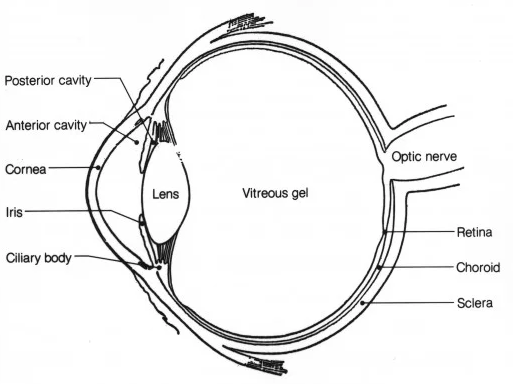
\includegraphics[width=\figwidth]{Sections/3AV1/Diagrams/eyediagram.png}
    \caption[Representation of an human eye]{Representation of an human eye \cite{AnatomyEyeHuman}}
    \label{fig:eye}
\end{figure}

Once the desired image is properly focused by the lens, an inverse version of it is shined on the aforementioned membrane, which is covered by two types of light sensitive cells, the \emph{cones} and \emph{rods}, which transform the observable image into a series of pulses, that get subsequently processed.

The cones are highly sensitive to color, being responsible for the \emph{photonic} or \emph{bright-light} vision. There are three different types of cones, corresponding to the wavelength they are susceptible to. These are the \emph{S}, \emph{M} and \emph{L} cones, being sensitive to, approximately, the blue, green and red light, respectively, making a somewhat similar capture to the RGB color system.

On the other side, rods aren't stimulated by bright light, being more active on low illumination levels. This aspect makes them responsible for giving a rough overview of the field of view. This is called as \emph{scotopic} or \emph{dim-light} vision. These cells are spread more broadly across the retina, while to the cones, which is also observable in the number of cells (approximately 6 million cones, to 100 million rods).

From this, it's already observable that the human visual system is more sensitive to differences on the luminosity, than to the color of an object \cite{mullenContrastSensitivityHuman1985}, which is a starting point for compressing video, as will be shown later in this chapter. However, many other opportunities come from the processing of the nerve signals, and the \emph{psychovisual} perception that follows.

Although more sensitive to \emph{luminance}, there is a threshold to which the difference between two objects --- $\Delta I$ --- can't be discerned. This relation is mentioned as \emph{contrast sensitivity function}, which is roughly approximated with the \emph{Weber's Law}

\begin{equation}
    \frac{\Delta I}{I}\approx constant
\end{equation}

Analyzing this equation, it's possible to conclude that the darker an object is, the lower the difference in luminance needs to be to distinguish another object. Also, darker images tend to be more susceptible to compression artifacts.

Besides the luminance values, the spatial and temporal frequencies also represent an important role in the perception of such errors. 

The image \ref{fig:noise} gives an example of the dependency with spatial frequency. The first image \ref{subfig:noiseOri} represents the original image, which got added with \gls{wgn}, represented in figure \ref{subfig:noise}. As it is observable, these artifacts are less noticeable on the highly detailed areas (branches and leafs of the tree) than in the smooth ones (sky in the top right corner). The effect of \emph{Weber's law} is also observed if we analyze the effect that the white noise as in the bright sun area, when compared to the darker areas.

\begin{figure}[h]
    \centering
    \begin{subfigure}[c]{\textwidth}
        \centering
        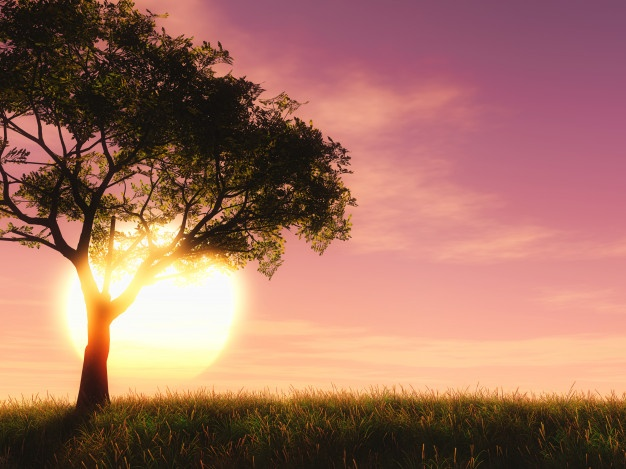
\includegraphics[width=\figwidth]{Sections/3AV1/Diagrams/paisagemOri.jpg}
        \caption{Original Image \cite{FreepikDownloadNow}}
        \label{subfig:noiseOri}
    \end{subfigure}
    \begin{subfigure}[c]{\textwidth}
        \centering
        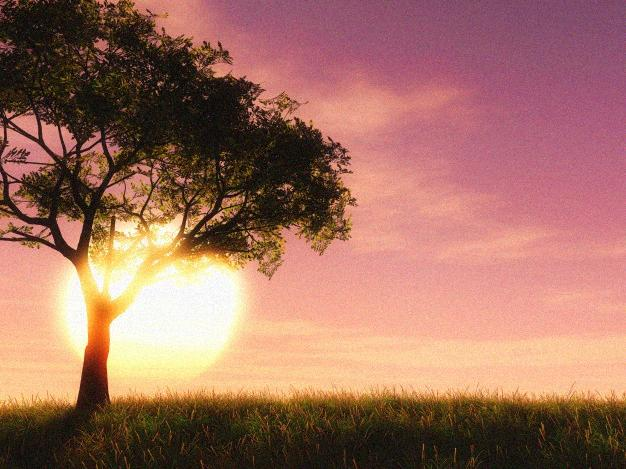
\includegraphics[width=\figwidth]{Sections/3AV1/Diagrams/paisagemNoise.jpg}
        \caption{Image with added WGN}
        \label{subfig:noise}
    \end{subfigure}
    \caption{Example of the effect of added noise on figure}
    \label{fig:noise}
\end{figure}

Temporal frequency dependency, although more challenging to exemplify, is easily understandable. On a sequence of frames with fast camera, or subject movements, the human eye doesn't have the ability to track details or other artifacts, while in slow moving scenes, it can easily identify errors.

These are some of the "\emph{flaws}" of the human visual system, that get exploited during the compression of video. However, other \emph{redundancies}, inherent from the captured images themselves contribute to the reduction of the video size, as will be described in the following sections.

%%%%%%%%%%%%%%%%%%%%%%%%%%%%%%%%%%%%%%%
\subsection{Redundancy Exploitation}

%\todo[inline,color=red!40]{*Types of redundancies (Temporal, Statistical and Coding)}
%\todo[inline,color=red!40]{*Color subsampling}
%\todo[inline,color=red!40]{*Intra-prediction}
%\todo[inline,color=red!40]{*Inter-prediction}
%\todo[inline,color=red!40]{*Transform and Quantization}
%\todo[inline,color=red!40]{*Entropy Coding}

Even though there are countless observable subjects and sceneries, it's unfair to think of a frame as a random sequence of pixels. Objects tend to represent clusters of pixels with roughly the same values, moving objects follow predictable directions, etc. Such characteristics represent redundancies that can be removed.

%%%%%%%%%%%%%%%%%%%
\subsubsection{Spatial Redundancy} \label{sssec:spatred}

Spatial redundancy comes from the similarity between neighboring pixels, on one frame. This aspect is easily verified through the autocorrelation of an image, as will be shown in the following example.

Taking image \ref{subfig:noiseOri} and calculating its autocorrelation with various horizontal shifts, gives origin to the graph in image \ref{fig:autocorr}.

\begin{figure}[h]
    \centering
    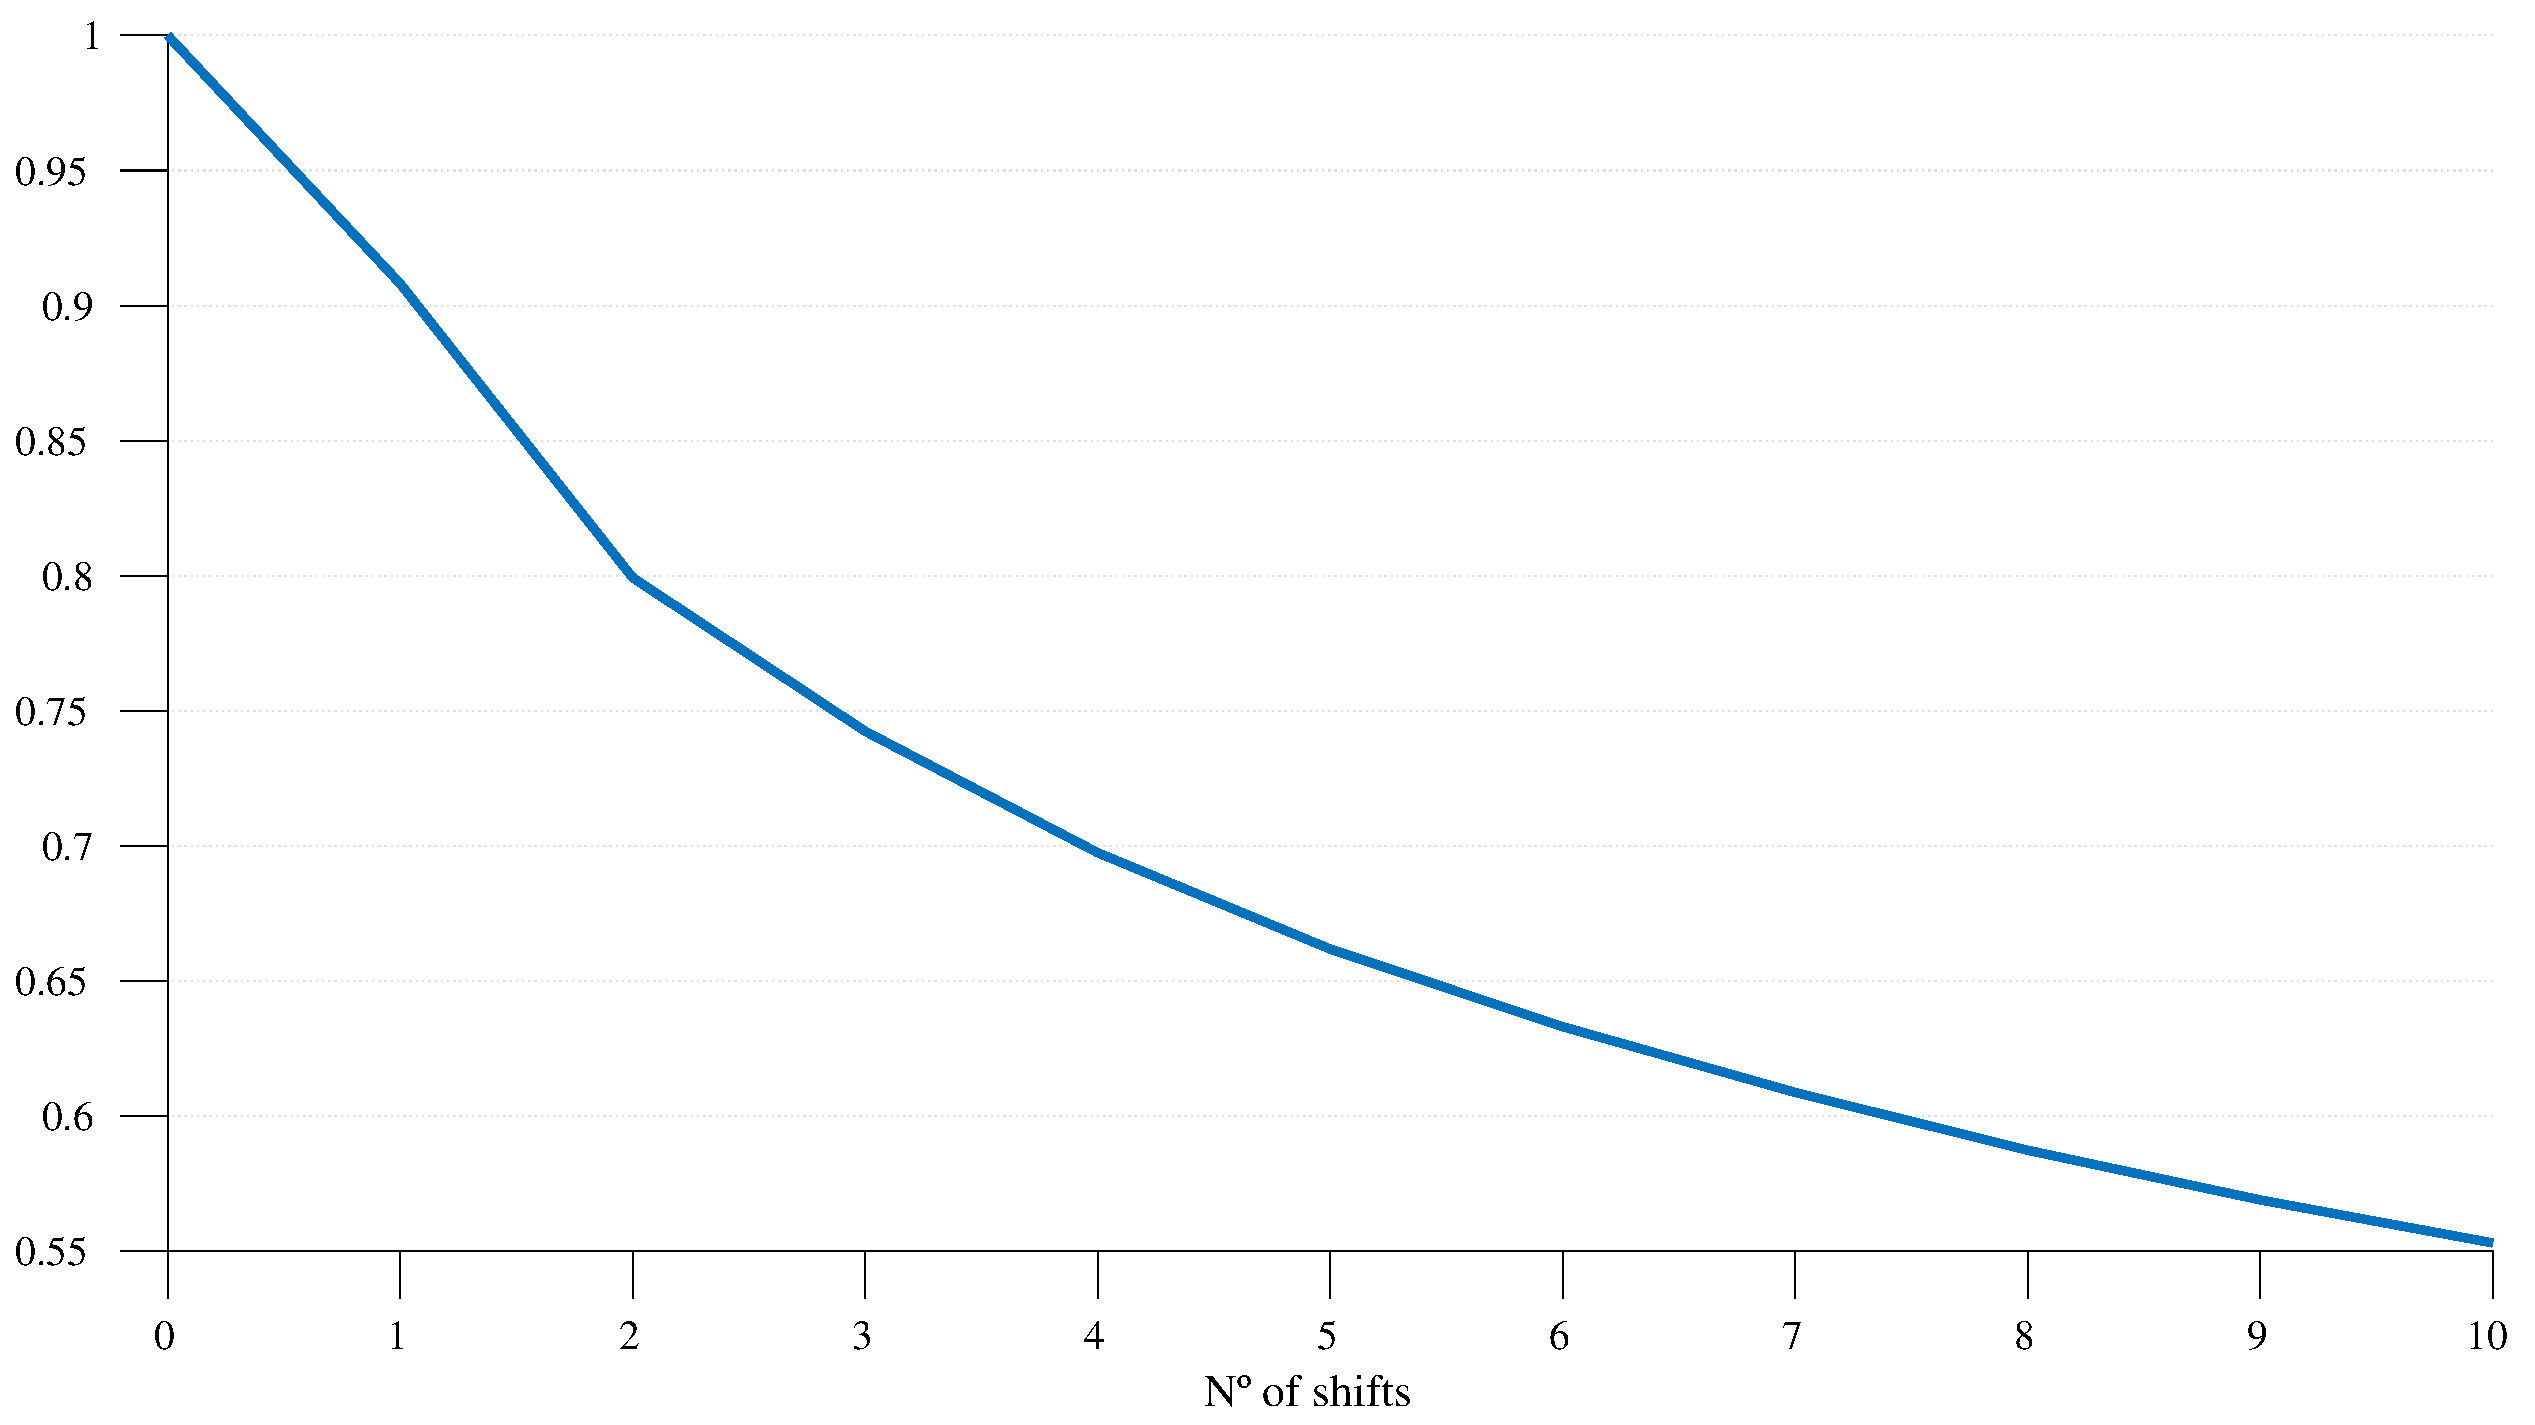
\includegraphics[width=\textwidth]{Sections/3AV1/Diagrams/intracorr.eps}
    \caption{Autocorrelation of image \ref{subfig:noiseOri}, with horizontal shifts}
    \label{fig:autocorr}
\end{figure}

As it is observable, for shorter shifts, the normalized autocorrelation is very close to 1, since most of the de-correlation comes for the mismatching edges. Although this relation varies depending on the image, it's safe to assume that it is very similar for the majority of the cases.

Such study gives a promising opportunity for compression, since it means that most pixels can be predicted from its neighbors. This aspect as lead to what now is known as \emph{differential} or \emph{predictive} coding.

On a video compression system, the spatial redundancy is considered in the \emph{intra-prediction} block, which calculates pixels, or pixel blocks, through its surrounds.

%%%%%%%%%%%%%%%%%%%
\subsubsection{Temporal Redundancy}

As expected, a series of consecutive frames, on the same subject, tend to be very similar between each other, especially if considered the $30$ or $60 fps$ desired nowadays. 

Making a similar analysis to what was made in section \ref{sssec:spatred}, a series of frames of the \emph{Stefan} sequence \cite{YUVSequences} was considered, and the cross correlation between the first and the following nine was calculated, giving origin to the graph in figure \ref{fig:crosscorr}.
\todor{verify graph generation}

\begin{figure}[h]
    \centering
    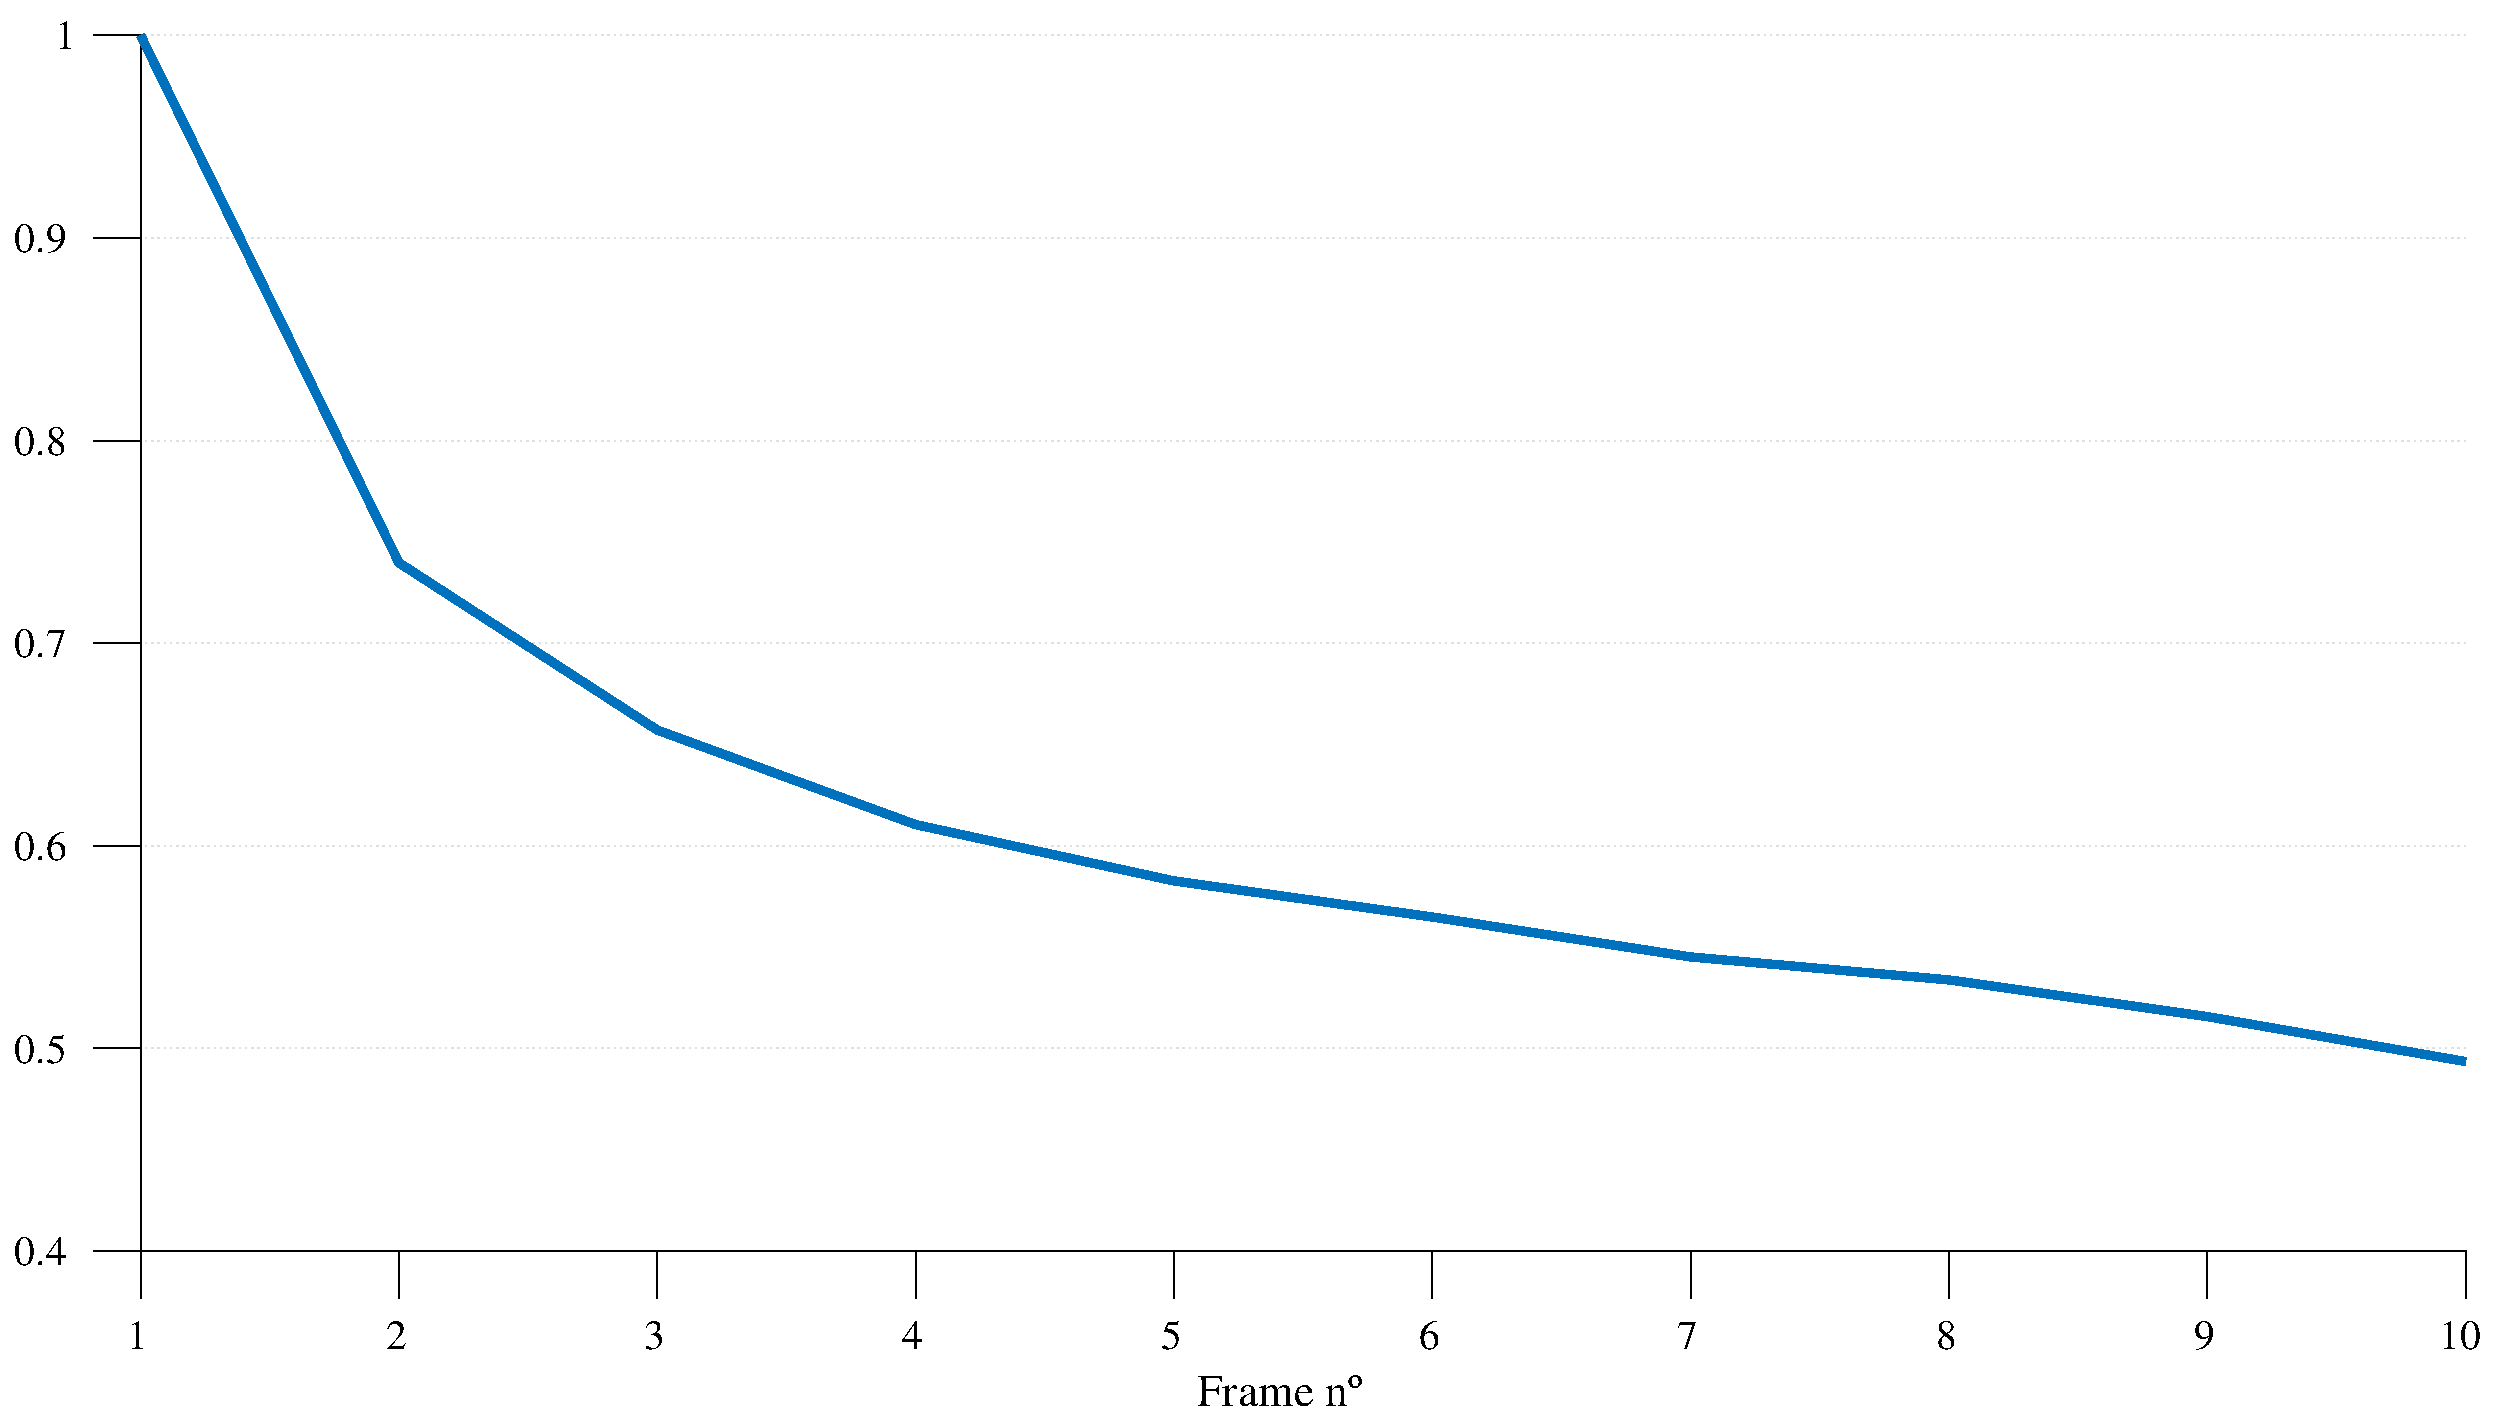
\includegraphics[width=\textwidth]{Sections/3AV1/Diagrams/intercorr.eps}
    \caption{Cross-correlation between the first and following nice frames of the \emph{Stefan} sequence}
    \label{fig:crosscorr}
\end{figure}

Similarly to what happened in the previous example, the cross correlation between consecutive frames is very high. Even though for faster moving scenes this relation might not be as pronounced, its application on video coding greatly contributes to the compression verified in the latest codecs. 

The codec takes advantage of this redundancy in the \emph{inter-prediction} stage, which is composed by the \emph{Motion Estimation} (MC) and \emph{Motion Compensation} (ME) blocks. On this stage, blocks of pixels in nearby frames are analyzed for movement, predicting its position for following frames.

%%%%%%%%%%%%%%%%%%%
\subsubsection{Psychovisual Redundancy}

From the redundancies presented in section \ref{ssec:hvs}, video codecs implement compression measures in various stages.

The first measure is the \emph{chroma subsampling}, which takes advantage of the lower perception to color, discarding some of the \emph{chroma} samples, depending on the subsampling chosen.

Typically, a pixel value is represented in one luminance and two chrominance values, on the \emph{YCbCr} color space. The subsampling is defined in through the relation of luminance to chroma samples, being the most common the 4:4:4, 4:2:2 and 4:2:0 standards, represented in figure \ref{fig:subsample}. In the first one, no chroma samples are discarded, which means that for each 4 luminance (\emph{Y}) samples, there are 4 \emph{Cb} and 4 \emph{Cr} samples. Correspondingly, in the second standard, for each 4 Y samples, only 2 of each color components are maintained. The last example, although its misleading term, means that only 1 of each 4 chroma samples are kept.

\begin{figure}[h]
    \centering 
        \begin{subfigure}[c]{\textwidth}
            \centering
            \begin{tikzpicture}[scale=0.75]    
    \coordinate (ycenter) at (2,3);
    \node[align=center] at (ycenter.north) {\textbf{Y}};
    \fill[gray!40] (0,0) rectangle (1,1);
    \fill[gray!70] (1,0) rectangle (2,1);
    \fill[gray!40] (2,0) rectangle (3,1);
    \fill[gray!70] (3,0) rectangle (4,1);
    \fill[gray!70] (0,1) rectangle (1,2);
    \fill[gray!40] (1,1) rectangle (2,2);
    \fill[gray!70] (2,1) rectangle (3,2);
    \fill[gray!40] (3,1) rectangle (4,2); 
    
    \coordinate (ccenter) at (7,3);
    \node[align=center] at (ccenter.north) {\textbf{Cb/Cr}};
    \fill[green!70!black] (5,0) rectangle (6,1);
    \fill[red!85!black] (6,0) rectangle (7,1);
    \fill[cyan] (7,0) rectangle (8,1);
    \fill[purple] (8,0) rectangle (9,1);
    \fill[blue!80!black] (5,1) rectangle (6,2);
    \fill[yellow!90!black] (6,1) rectangle (7,2);
    \fill[orange] (7,1) rectangle (8,2);
    \fill[brown] (8,1) rectangle (9,2);

\end{tikzpicture}
            \caption{4:4:4}
            \label{subfig:444}
        \end{subfigure}
        \begin{subfigure}[c]{\textwidth}
            \centering
            \begin{tikzpicture}[scale=0.75]    
    \coordinate (ycenter) at (2,3);
    \node[align=center] at (ycenter.north) {\textbf{Y}};
    \fill[gray!40] (0,0) rectangle (1,1);
    \fill[gray!70] (1,0) rectangle (2,1);
    \fill[gray!40] (2,0) rectangle (3,1);
    \fill[gray!70] (3,0) rectangle (4,1);
    \fill[gray!70] (0,1) rectangle (1,2);
    \fill[gray!40] (1,1) rectangle (2,2);
    \fill[gray!70] (2,1) rectangle (3,2);
    \fill[gray!40] (3,1) rectangle (4,2); 
    
    \coordinate (ccenter) at (7,3);
    \node[align=center] at (ccenter.north) {\textbf{Cb/Cr}};
    \fill[green!70!black] (5,0) rectangle (6,1);
    \fill[green!70!black] (6,0) rectangle (7,1);
    \fill[cyan] (7,0) rectangle (8,1);
    \fill[cyan] (8,0) rectangle (9,1);
    \fill[blue!80!black] (5,1) rectangle (6,2);
    \fill[blue!80!black] (6,1) rectangle (7,2);
    \fill[pink] (7,1) rectangle (8,2);
    \fill[pink] (8,1) rectangle (9,2);

\end{tikzpicture}
            \caption{4:2:2}
            \label{subfig:422}
        \end{subfigure}
        \begin{subfigure}[c]{\textwidth}
            \centering
            \begin{tikzpicture}[scale=0.75]    
    \coordinate (ycenter) at (2,3);
    \node[align=center] at (ycenter.north) {\textbf{Y}};
    \fill[gray!40] (0,0) rectangle (1,1);
    \fill[gray!70] (1,0) rectangle (2,1);
    \fill[gray!40] (2,0) rectangle (3,1);
    \fill[gray!70] (3,0) rectangle (4,1);
    \fill[gray!70] (0,1) rectangle (1,2);
    \fill[gray!40] (1,1) rectangle (2,2);
    \fill[gray!70] (2,1) rectangle (3,2);
    \fill[gray!40] (3,1) rectangle (4,2); 
    
    \coordinate (ccenter) at (7,3);
    \node[align=center] at (ccenter.north) {\textbf{Cb/Cr}};
    \fill[blue!80!black] (5,0) rectangle (6,1);
    \fill[blue!80!black] (6,0) rectangle (7,1);
    \fill[pink] (7,0) rectangle (8,1);
    \fill[pink] (8,0) rectangle (9,1);
    \fill[blue!80!black] (5,1) rectangle (6,2);
    \fill[blue!80!black] (6,1) rectangle (7,2);
    \fill[pink] (7,1) rectangle (8,2);
    \fill[pink] (8,1) rectangle (9,2);

\end{tikzpicture}
            \caption{4:2:0}
            \label{subfig:420}
        \end{subfigure}
       \caption{Representation of chroma subsampling}
    \label{fig:subsample}
\end{figure}

From the reduced sensitivity to details (or areas with high spatial frequency), the compression is explored in the \emph{Transform} (T) and \emph{Quantization} (Q) blocks. In the first stage, blocks of pixels are evaluated in their frequency components. These are then evaluated in the second stage, where the least significant ones get discarded. In the decoder, the image is reconstructed with the maintained coefficients, without much impact to the image quality. This process is further explained throughout the work.

On the Quantization block, some work was also developed to account for \emph{Weber's law}, where the quantization depends on the average luminance value of the block. This concept was first introduced in \cite{watsonEfficiencyModelHuman1988}, and since then experimented in various codecs, such as HEVC \cite{rouisPerceptualVideoContent2018}.

%%%%%%%%%%%%%%%%%%%
\subsubsection{Coding Redundancy}

Coding redundancy is directed to the method of representing information in the digital domain, i.e., the bits themselves, and how they are organized.

It is known that symbol probability plays a major role in information compression, across a wide variety of branches, and video is no exception. Taking this into account, codecs take advantage of coding redundancy in the \emph{Entropy Encoder} stage.

%%%%%%%%%%%%%%%%%%%%%%%%%%%%%%%%%%%%%%%
\subsection{Basic Video Compression/Decompression System}

\todo[inline,color=red!40]{*Encoder Model}
\todo[inline,color=red!40]{*Decoder Model}

From the basic principles of the previously mentioned blocks, it is possible to integrate them into two complete compression --- \emph{Encoder} --- and decompression --- \emph{Decoder} --- modules.

%%%%%%%%%%%%%%%%%%%
\subsubsection{Encoder Model}

\begin{figure}[!htbp]
    \centering
    \begin{tikzpicture}[%
    >=triangle 60,              % Nice arrows; your taste may be different
    start chain=going right,    % General flow is top-to-bottom
    node distance=2.5cm,          % Global setup of box spacing
    every join/.style={norm},   % Default linetype for connecting boxes
    scale=0.7, every node/.style={transform shape}
    ]

\tikzset{
    base/.style={draw, on chain, on grid, align=center},
    proc/.style={base, rectangle, text width=1.6cm, fill=black!15, minimum height=1.5cm, minimum width=1.5cm,font={\bfseries}},    
    frame/.style={base, minimum height=1.5cm, minimum width=2cm, fill=blue!10, thick},
    sub/.style={base, circle, inner sep=0pt, radius=0.4cm, fill=black!10, minimum height=3.5ex, font={\bfseries}},
    spot/.style={circle, inner sep=0pt, radius=0.4cm, minimum height=2mm, draw},
    edge rectangle/.style={ to path={ rectangle (\tikztotarget)}},
    % coord node style is used for placing corners of connecting lines
    coord/.style={coordinate, on chain, on grid, node distance=6mm and 40mm},
    % Arrows 
    fforw/.style={->, thick},
    fback/.style={->, thick, red!75!black},
    aref/.style={<->, dashed, black!50},
    % -------------------------------------------------
    % Connector line styles for different parts of the diagram
    cascaded/.style = {%
    general shadow = {%
      shadow scale = 1,
      shadow xshift = -1ex,
      shadow yshift = 1ex,
      draw,
      thick,
      fill = blue!40},
    general shadow = {%
      shadow scale = 1,
      shadow xshift = -.5ex,
      shadow yshift = .5ex,
      draw,
      thick,
      fill =blue!40},
    fill = blue!40, 
    draw,
    thick,
    minimum width = 2cm,
    minimum height = 1.5cm},
    base
}    

%% Top row
\node [frame] (inframe) {Input\\Frame};
    \node [coord] (ni1) {};    
    \node [coord, right=2mm of inframe.east] (ni2) {};
\node [sub, right=2cm of ni1] (sub) {-};
    \draw [fforw] (inframe) -- (sub);
\node [proc] (T) {T};
    \draw [fforw] (sub) -- (T);
\node [proc] (Q) {Q};
    \draw [fforw] (T) -- (Q);
\coordinate (rq) at ($(Q.east)+(4mm,0)$);
\node [proc, right=1cm of Q.east] (EC) {Entropy\\Coding};
    \draw [fforw] (Q) -- (EC);
\coordinate (out) at ($(EC.east)+(4mm,0)$);
%\path (EC) to node [yshift=-1em] {Encoded\\Bitstream} (out);
    \draw [fforw] (EC) -- (out);

%% Reference
\node [cascaded, below=5cm of inframe] (ref) {Reference\\Frames};

%% Intra
\node [proc, below=1.5cm of ni1] (intra) {Intra\\Coding};
    \coordinate (ni3) at (ni2 |- intra);    
    \draw [fforw] (ni3) -- (intra);

%% Inter    
\node [proc,right=of ref] (inter) {Inter\\Coding};
    \node [coord, below=4.5cm of ni2] (ni4) {};
    \draw [fforw] (ni2) -- (ni4) |- ($(inter.west)+(0,5mm)$);
    \draw [fforw] ($(ref.east)+(0,-5mm)$) -- ($(inter.west)+(0,-5mm)$);

%% Selector
\coordinate (rintra) at ($(intra.east)+(5mm,0)$);
\node [spot, below=1cm of rintra, fill=black] (sintra) {};
    \draw [thick] (intra.east) -- (rintra) |- (sintra.north);

\coordinate (rinter) at ($(inter.east)+(5mm,0)$);
\node [spot, above=1cm of rinter, fill=black] (sinter) {};
    \draw [thick] (inter.east) -- (rinter) |- (sinter.south);

\path (sintra) -- (sinter) coordinate [midway] (intraintermid);
\node [spot, at=(sub |- intraintermid)] (sel) {};
\draw [dashed] ($(sel)+(-4mm,3.3mm)$) arc (140:220:5mm);
    \draw [fforw] (sintra) -- (sel);
    \draw [fforw] (sel) -- (sub);

%% Lower Row    
\node [sub, below=3.7cm of sel] (add) {+};
    \draw [fback] (sel) -- (add);
\node [proc] (T1) {$\mathbf{T^{-1}}$};
    \draw [fback] (T1) -- (add);
\node [proc] (Q1) {$\mathbf{Q^{-1}}$};
    \draw [fback] (Q1) -- (T1);
\coordinate (rq1) at ($(Q1.east)+(4mm,0)$);
    \draw [fback] (rq) -- (rq1) |- (Q1);
\node [frame, below=7.4cm of inframe] (recframe) {Reconstructed\\Frame};
    \draw [fback] (add) -- (recframe);
\end{tikzpicture}
    \caption{Basic Encoder Model}
    \label{fig:basicenc}
\end{figure}

%%%%%%%%%%%%%%%%%%%%%%%%%%%%%%%%%%%%%%%%%%%%%%%%%%%%%%%%%%%%%%%%%%%%%%%%%%%%%%
\section{Previous Standards}

\todo[inline,color=red!40]{*Previous generations}

%%%%%%%%%%%%%%%%%%%%%%%%%%%%%%%%%%%%%%%%%%%%%%%%%%%%%%%%%%%%%%%%%%%%%%%%%%%%%%
\section{AV1}

\todo[inline,color=red!70]{\textbf{Review \textit{AV1 Bitstream and Decoding Process}}}
\todo[inline,color=red!40]{*Development Process}
\todo[inline,color=red!40]{*AOMedia companies}
\todo[inline,color=red!40]{*Comparation with past generations}
\todo[inline,color=red!40]{*Introduction of modules not present on other video codecs}
\todo[inline,color=red!40]{*Block diagram}

\input{Sections/3AV1/Diagrams/av1block.tex}

%%%%%%%%%%%%%%%%%%%%%%%%%%%%%%%%%%%%%%%%%%%%%%%%%%%%%%%%%%%%%%%%%%%%%%%%%%%%%%
\section{Performance Analysis}

\todo[inline,color=red!40]{*Compression gains}
\todo[inline,color=red!40]{*Quality assessment}
\todo[inline,color=red!40]{*Complexity (general/modules) and timing issues}

\clearpage
\printbibliography[heading=subbibliography]
\addcontentsline{toc}{section}{References}